% \begin{center}
\clearpage
\phantomsection
\cftaddtitleline{toc}{chapter}{Chapter 1 -- chapter one title here}{3}
% this is not ideal as I need to manually write the page number....
% commands below give wrong page numbers in TOC (+/- 1 page) ...
% \addcontentsline{toc}{chapter}{Chapter 1 -- Drivers of observed biotic homogenization in pine barrens of central Wisconsin}
% \par\end{center}

% \resetlinenumber
\begin{center}
\textbf{\Large{}Chapter 1 -- chapter one title here}
\label{chap:chapter1}
\par
\end{center}
{\Large \par}

\bigskip{}


\begin{center}
Author 1 and Author 2 % authors
\par\end{center}

\bigskip{}



\lyxaddress{Department of Botany, University of Wisconsin-Madison, Madison, WI,
53706 USA}

% if necessary
Citation:
\begin{quote}
Authors. 2015. Title. Journal. 96:1030\textendash 1041
\end{quote}
\vfill
\chapter*{}
\setcounter{chapter}{1}
% \label{chap:taxonomic_changes}
% \clearpage{}

\textbf{Abstract:}

Fire suppression throughout the twentieth century greatly altered
plant communities in fire-dominated systems across North America.
... Our findings highlight the key role fire plays in shaping
the assembly of these pine-barrens communities.

\textbf{\emph{Key words}}\emph{: plant community change, ..., Wisconsin.}

\clearpage{}


\phantomsection\addcontentsline{toc}{section}{Introduction}
\section*{Introduction}

Anthropogenic and natural disturbances profoundly affect biodiversity
and ecosystem functions \citep{naeem2009biodiversity}.

\phantomsection\addcontentsline{toc}{section}{Methods}
\section*{Methods}

\subsection*{Study sites and area}

The CSP covers $885,800$ ha, representing $6.1\%$ of the land area
of the Wisconsin state.

\phantomsection\addcontentsline{toc}{section}{Results}
\section*{Results}
\subsection*{Changes in community structures}

Over the past 54 years, tree density has decreased 24\% (from 724
to 550 \emph{trees/ha}; paired-$t_{29}=-3.31$, $p=0.003$) while
the average DBH per stem has increased 15\% (from 19 to 22 $cm$/\emph{tree};
paired-$t_{29}=3.94$ , $p=0.0004$).

\phantomsection\addcontentsline{toc}{section}{Discussion}
\section*{Discussion}

In this study, we documented ...

\subsection*{Acknowledgments}

We thank...

\clearpage{}
% \nocite{*}
\phantomsection\addcontentsline{toc}{section}{References}
\begin{onehalfspace}
\bibliographystyle{ecology}
\bibliography{chapter1/ch1}
\end{onehalfspace}


\renewcommand{\tablename}{Table}
\renewcommand{\thetable}{\arabic{table}}
\renewcommand{\figurename}{Figure}
\renewcommand{\thefigure}{\arabic{figure}}
\setcounter{figure}{0}
\setcounter{table}{0}

\clearpage{}
\phantomsection\addcontentsline{toc}{section}{Tables}
\section*{Tables:}
\vspace{60pt}

\begin{table}[h]
\begin{centering}
\doublespacing\caption{\label{tab:changes-in-rel-frequency}Results of changes .\protect \\
}
\par\end{centering}

\centering{}\doublespacing%
\begin{tabular*}{1\textwidth}{@{\extracolsep{\fill}}clccc}

\toprule
 &  & \multicolumn{2}{c}{Mean relative quadrat frequency ($\pm$ SD)} & \multicolumn{1}{c}{}\tabularnewline
\cline{3-4}
 &  & 1958 & 2012  & \multicolumn{1}{c}{\emph{P}-{\small{}value}}\tabularnewline
\midrule
\multicolumn{2}{l}{Plant growth habit} &  &  & \tabularnewline
 & Forb & 0.461($\pm$0.083) & 0.284($\pm$0.066) $\downarrow$ & $p<0.0001$\tabularnewline
 & Fern /fern ally & 0.004($\pm$0.008) & 0.017($\pm$0.020) $\uparrow$ & $p=0.0004$\tabularnewline
 & Graminoid & 0.065($\pm$0.100) & 0.124($\pm$0.069) $\uparrow$ & $p=0.0058$\tabularnewline
 & Woody & 0.467($\pm$0.110) & 0.574($\pm$0.059) $\uparrow$ & $p<0.0001$\tabularnewline
\multicolumn{2}{l}{Plant origin} &  &  & \tabularnewline
 & Exotic & 0.007($\pm$0.026) & 0.017($\pm$0.033) $\uparrow$ & $p=0.061$\tabularnewline
 & Native & 0.993($\pm$0.026) & 0.983($\pm$0.033) $\downarrow$ & $p=0.061$\tabularnewline
\bottomrule
\end{tabular*}
\end{table}

\clearpage{}

\phantomsection\addcontentsline{toc}{section}{Figures}
\noindent\textbf{Figures:}

\noindent \textbf{Figure 1.} Map of the 30 study sites in the central
sand plains of Wisconsin.

\begin{figure}
\centering{}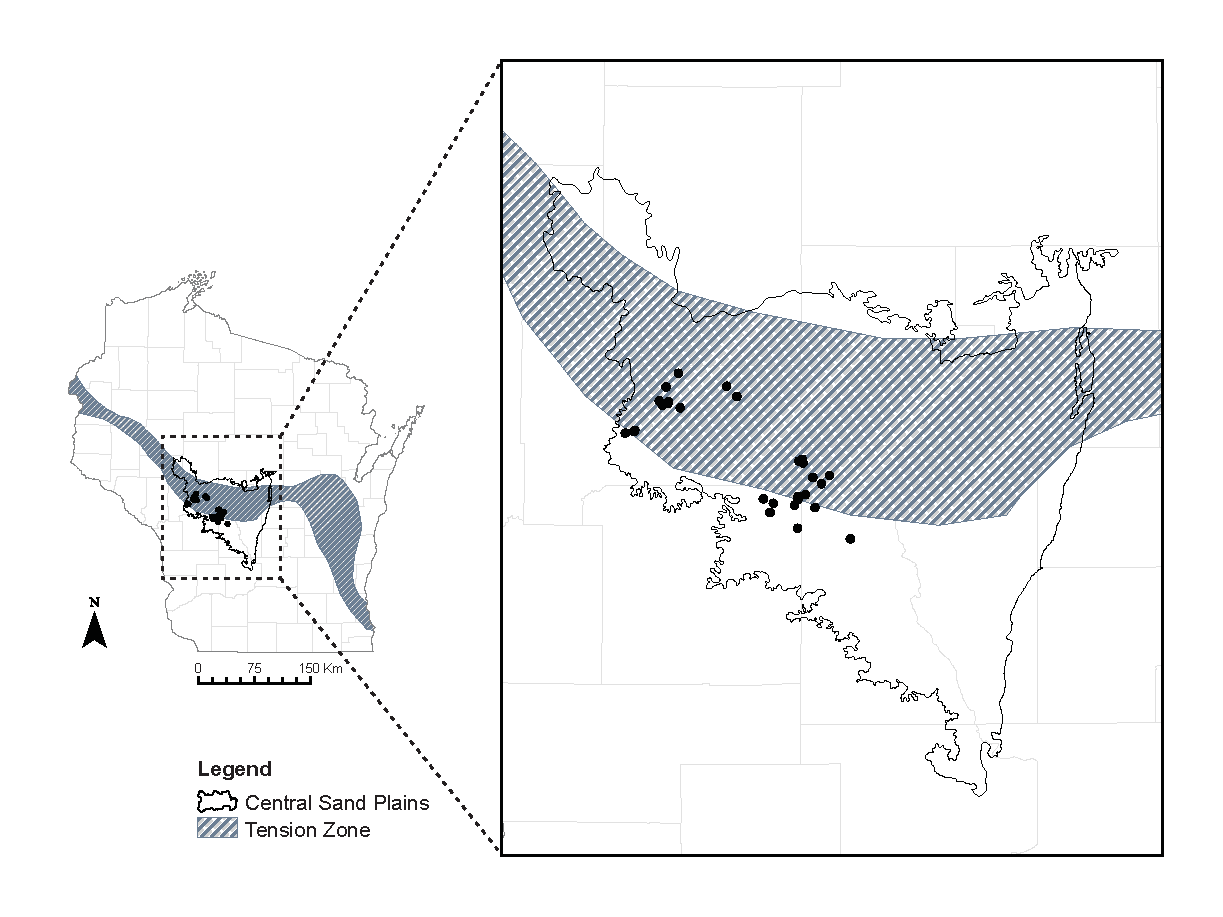
\includegraphics[width=0.9\textwidth]{chapter1/figures-maintext/map_20140214.pdf}\caption{\label{fig:Reampled-sites-in} Map of the 30 study sites in the central sand plains of Wisconsin.}
\end{figure}


\clearpage{}

\appendix

%\newcommand{\tablename0}{\tablename}
%\newcommand{\thetable0}{\thetable}
%\newcommand{\figurename0}{\figurename}
%\newcommand{\thefigure0}{\thefigure}
\renewcommand{\tablename}{\textsc{Table}}
\renewcommand {\thetable}{\textbf{A\arabic{table}}}
\renewcommand{\figurename}{\textsc{Fig.}}
\renewcommand {\thefigure}{\textbf{A\arabic{figure}}}
\setcounter{figure}{0}
\setcounter{table}{0}

\setlength{\tabcolsep}{2pt}
\LTcapwidth=\textwidth

\begin{onehalfspace}
\begin{longtable}[h]{p{0.02\textwidth}p{0.35\textwidth}p{0.1\textwidth}p{0.1\textwidth}p{0.1\textwidth}p{0.1\textwidth}p{0.15\textwidth}}
\caption{Results of indicator species analysis.}\\

\toprule

 & Taxon & Site \#(1958) & Site \#(2012) & Quadrat \%(1958) & Quadrat \%(2012) & Status\\
 \hline
\endfirsthead
\hline
& Taxon & Site \#(1958) & Site \#(2012) & Quadrat \%(1958) & Quadrat \%(2012) & Status\\
\hline
 \endhead
 \hline
\multicolumn{7}{r}{continued in next page\dots} \\
\endfoot
\bottomrule
\endlastfoot

1 & \emph{Acer rubrum } &  21 &  30 & 31.67 & 63.87 & winner \\
  2 & \emph{Achillea millefolium } &   7 &   1 & 1.67 & 0.07 & loser \\
  3 & \emph{Amelanchier spp } &  14 &  23 & 5.00 & 8.27 & winner \\
  4 & \emph{Andropogon gerardii } &   6 &   1 & 4.83 & 0.53 & not change \\
  5 & \emph{Anemone quinquefolia}  &   3 &   9 & 0.83 & 2.93 & winner \\
  6 & \emph{Antennaria spp } &  12 &   1 & 5.33 & 0.07 & loser \\
  7 & \emph{Apocynum androsaemifolium } &  18 &  18 & 6.17 & 4.67 & not change \\
  8 & \emph{Aralia nudicaulis } &  13 &  14 & 8.33 & 3.53 & not change \\
  9 & \emph{Arctostaphylos uva-ursi}  &   3 &   1 & 1.50 & 0.07 & not change \\
  10 & \emph{Aronia melanocarpa}  &   0 &  22 & 0.00 & 10.00 & winner \\
  \end{longtable}
\end{onehalfspace}

\begin{figure}
\begin{centering}
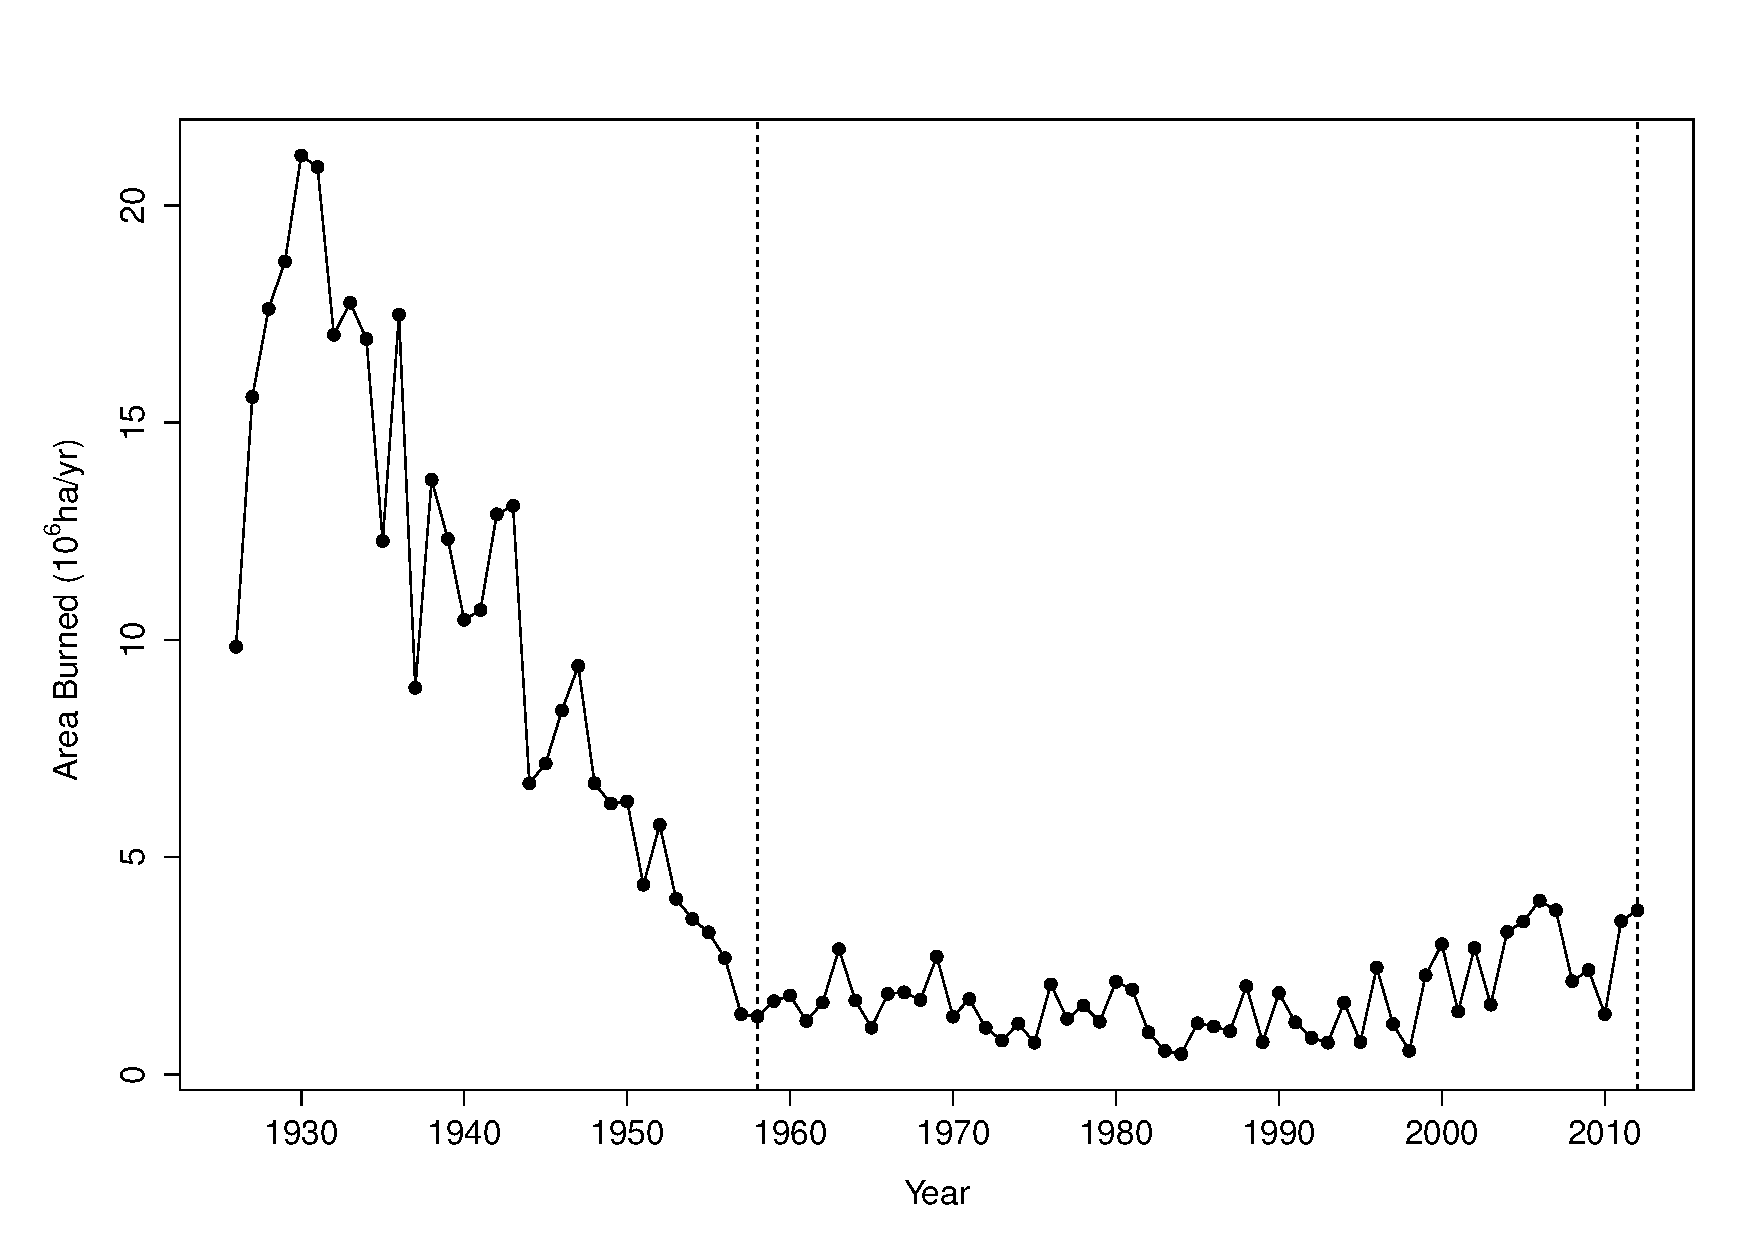
\includegraphics[width=1\textwidth]{chapter1/figures-appendix/fire.pdf}
\par\end{centering}
\caption{\label{fig:Fire-burning-extent}Fire burning extent in the United
States in millions of hectares per year from 1926 to 2012.}
\end{figure}

% so next chapter's figure/table names will be normal
\renewcommand{\tablename}{Table}
\renewcommand{\thetable}{\arabic{table}}
\renewcommand{\figurename}{Figure}
\renewcommand{\thefigure}{\arabic{figure}}
\clearpage
